\section{Resistor Circuits}

In this lab you will study the relationships between voltage, current, and resistance in simple DC circuits.

\vspace{\baselineskip}

Safety: electricity does have the ability to cause harm, but this lab should be very safe as long as you follow the instructions and don’t do anything stupid (e.g. take apart a power supply). 

\vspace{\baselineskip}

\underline{\textbf{Part 1}} \par
See https://phet.colorado.edu/sims/html/circuit-construction-kit-dc/latest/circuit-construction-kit-dc\_en.html for practice

\vspace{\baselineskip}

The DC power supplies at your lab stations are basically batteries with knobs so you can change the voltage.
Make sure your power supply is initially turned off (the switch may be in the back) and the knob is turned all the way down.
If it's not plugged in, plug it in and then turn it on and adjust the knob so the voltage is about 5V. 

\vspace{\baselineskip}

Take out your multi-meter and set it to voltage mode and measure the voltage of the power supply. It should read ~5V.

\vspace{\baselineskip}

The diagram below shows a standard breadboard layout:

\begin{figure}[H]
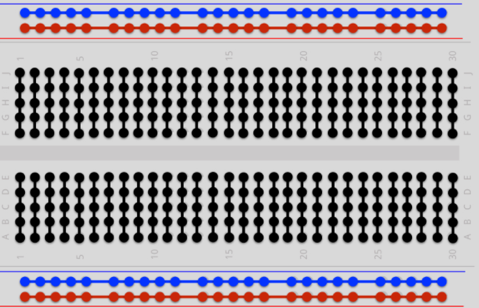
\includegraphics[scale=0.80]{figures/resistor-circuits/breadboard.png}
\end{figure}

The top 2 and bottom 2 rows (red (+) and blue (-)) are typically used for connecting to your power supply while the middle (black) is for plugging in circuit components.
Attempt to construct the following circuit:

\begin{figure}[H]
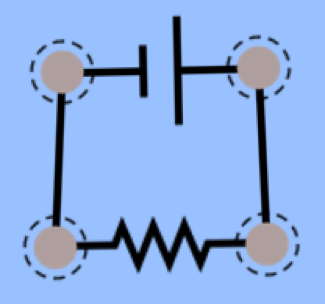
\includegraphics[scale=0.80]{figures/resistor-circuits/one-resistor.png}
\end{figure}

Have your instructor check your circuit before proceeding.
Next measure the voltage across the resistor and the current through the resistor.
Make sure your multi-meter is in the correct mode and that you connect it correctly.
Doing this incorrectly can blow a fuse in the multi-meter.
Note that measuring current requires you to break the circuit and put the meter in series with the resistor while measuring voltage requires you to put the meter in parallel with the resistor.
See below.

\begin{figure}[H]
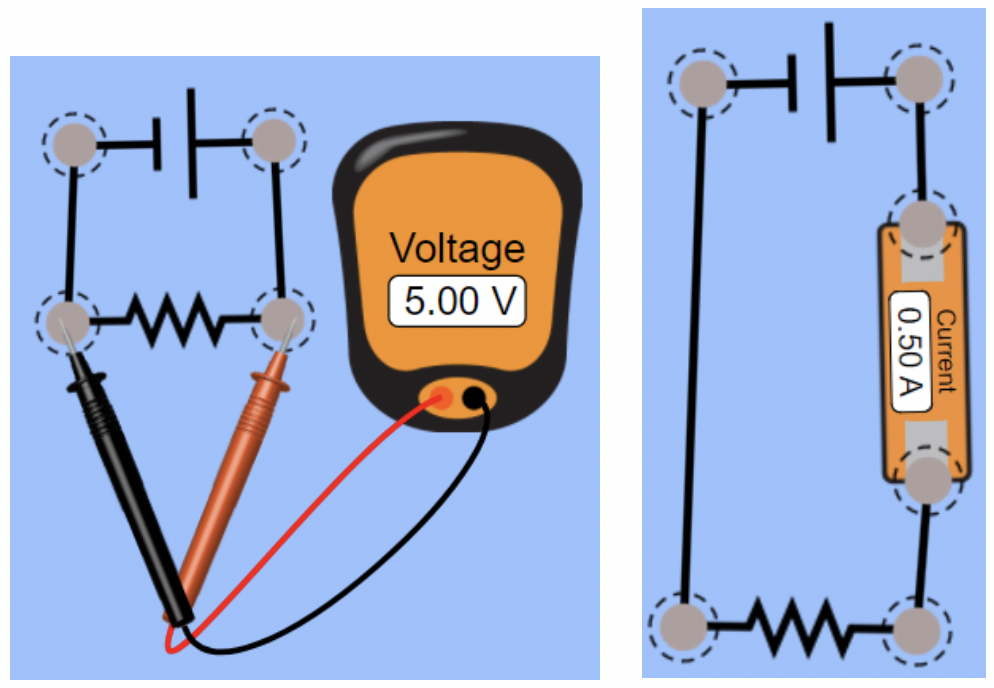
\includegraphics[scale=0.55]{figures/resistor-circuits/V-I-measurement.png}
\end{figure}

\underline{\textbf{Part 2}} \par

With your 5V power supply, construct the circuit below.
You may use your multi-meter to measure the resistance of the resistors rather than rely on the colored bands.
Calculate and then measure the voltage across and current through each resistor.
Also calculate and measure the equivalent resistance of the 3 resistor system.
Remember to be careful not to blow a fuse in the multi-meter!

\begin{figure}[H]
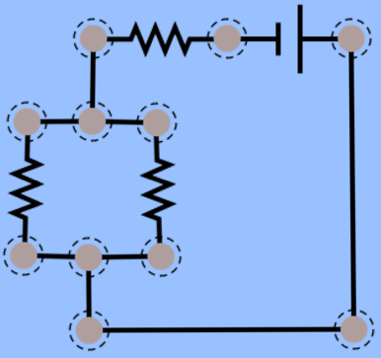
\includegraphics[scale=0.90]{figures/resistor-circuits/mixed-circuit.png}
\end{figure}

\pagebreak \clearpage
